%!TEX root = thesis.tex 

\chapter{Implementation} \label{cha:Implementation}
	\paragraph{}
	In Chapter \ref{cha:An Alternative Approach} we defined a set of requirements for our ideal tool and in Chapter \ref{cha:The Tool} we continued to describe our approach to achieve those requirements. Now that we have established our approach we can take this high level design and create a working implementation for it. In this chapter we will explain how we implemented our design and go into more detail on the important choices we had to make. Next, we will go over each major component of our tool and describe the technical aspect in more detail. Finally we will list some important issues we ran into when designing and developing our tool and we will suggest some work around or solutions.
	\section{Data Management} \label{sec:Data Management}
	\paragraph{}
	In our local JavaScript database we will create a simplified version of the RSL~\cite{SignerDOC}~\cite{Signer2007} model. Our tool is designed to work on web resources so there is no need to support additional media types. We will make sure that the local database is compatible with the actual RSL model to make extending the tool to an external RSL server fast and painless. In this section we will give a short description of the local database.
	\paragraph{}
	The \code{Resource} table contains the web resources that can be linked to and is identified by a resource descriptor, in our case this is the URL of the web resource, which will be the same in an RSL database. A \code{Selector} table is linked to the resources and defines the part of the document that will be selected as the source or destination of a hyperlink, in our case the selectors will be defined by an Xpointer on the web page. The \code{Selector} table also keeps a reference to the associated resource. Finally we have the hyperlinks themselves which are saved in two separate tables one table contains the sources of the hyperlinks, while the second table contains the destinations. This will allow us to easily save hyperlinks with multiple destinations and multiple sources. Both of the tables will have a field with a number that identifies the hyperlink. That way we can actually combine the information from both tables. We will also keep a \code{Hyperlink} table that joins the both the destinations and the sources. In this table we can also add more information such as the creator of the hyperlink or the date on which it was created.
	\paragraph{}
	These five tables will provide a means to save all hyperlinks in our simplified version of the an RSL database. In Chapter \ref{cha:An Alternative Approach} we discussed the need for tags on our metadata as well. To save this additional information we need an extra table named \code{Tag}. Tags will be saved in a separate table, and when a selector is created with a tag this information is saved in a join table \code{Selector\_Tag}. When a new tag is used that did not exist yet, a new entry is added in the Tag table. The amount of times a tag is used is then easily calculated from this table and this gives us an easy way to provide the users with a list of already existing tag names.
	\paragraph{}
	With this database in place we are able to store all the information we need to create the hyperlinks between different resources. This database is also compatible with the RSL model so migrating the data to a remote database poses no real difficulty.
	\begin{figure}[h]
		\centering
		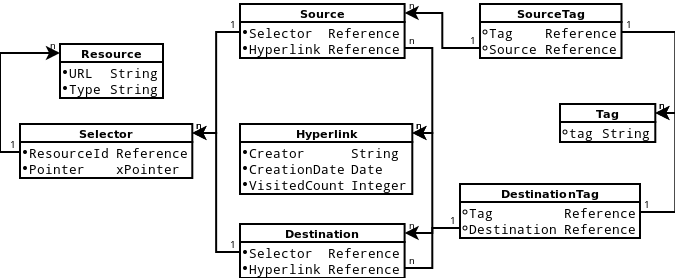
\includegraphics[width=\textwidth]{implementation/database.png}
		\caption{Model Of Local JS Database}
	\end{figure}
	\paragraph{}
	The implementation of this database will be done using HTML5 local storagei, this local storage is a simplified version of SQLite~\cite{owens2006definitive} implemented in JavaScript.
	\paragraph{}
	To make our life easier in the future we start with creating a \code{Database} prototype for which we can define methods to handle the communication with the low level database.
	\begin{lstlisting}[language=JavaScript]
var Database = function(){
	var myDb = false;
}
	\end{lstlisting}
	We can now define our methods on this database prototype
	\begin{lstlisting}[language=JavaScript]
Database.prototype.SomeMethod = function() {
	...
}
	\end{lstlisting}
	\paragraph{Set-up}
	The first thing we need to do is create a client side database if the database not yet exists so we define the \code{initDB} method as follows
	\begin{lstlisting}[language=JavaScript]
Database.prototype.initDB = function() {
	try {
		if (!window.openDatabase) {
			alert('Databases are not supported in this browser.');
		} else {
			var shortName = 'DEMODB';
			var version = '1.0';
			var displayName = 'DEMO Database';
			var maxSize = 1000000; // in bytes
			this.myDb = openDatabase(shortName, version, displayName, maxSize); //creation of DB
			this.createTables();
		}
	} catch(e) {

		if (e == 2) {
			// Version number mismatch.
			console.log("Invalid database version.");
		} else {
			console.log("Unknown error "+e+".");
		}
		return;
	}
}
	\end{lstlisting}
	\paragraph{}
	Running \code{Database.initDB()} creates the database and already makes a call to \code{Database.createTables()} which is defined as follows
	\begin{lstlisting}[language=JavaScript]
Database.prototype.createTables = function(){
	this.myDb.transaction(
		function (transaction) {
			var queries = [
				  'CREATE TABLE IF NOT EXISTS tableName('
						 ... //table column definitions
				+ ');']
			for (var i = 0; i < queries.length; i++) {
				transaction.executeSql( queries[i], [], this.nullDataHandler, this.errorHandler);
			};
		}
	);
}
	\end{lstlisting}
	\paragraph{}
	As we can see, the database framework makes use of transactions that are called on the database using a callback function. The database framework uses these transaction callbacks because the database is queried asynchronously. This means that when we launch a query in our code we will not get a response in the same way a desktop application would from a MySQL\cite{dubois2008mysql} database, instead the executing of the program continues independents of when the query will produce a result but when the query finishes the callback is then called on the result. 
	\paragraph{}
	In the previous snippet the \code{nullDataHandler} and \code{errorHandler} are both callback functions and are called when respectively the query succeeds, or fails. Since we do not need to execute any code once the tables are created we provide the \code{nullDataHandler} which just returns.
	\begin{lstlisting}[language=JavaScript]
Database.prototype.nullDataHandler = function (transaction, results) {
	console.log(results);
}
Database.prototype.errorHandler = function (transaction, error) {
	alert("Error processing SQL: "+error);
	return true;
}
	\end{lstlisting}

	\paragraph{}
	To send a query to the database we use the \code{executeSql} function as shown earlier. The following code allows us to select all the selectors that are defined on a single resource
	\begin{lstlisting}[language=JavaScript]
Database.prototype.getSelectors = function(resourceIdentifier, callback){
	var db = this;
	this.Db.transaction(
		function (transaction){
			transaction.executeSql("SELECT * FROM selector where resourceId = ? ;", [resourceIdentifier], db.resultHandler(callback));
		}
	)
}
	\end{lstlisting}
	\paragraph{}
	When we call this function we can provide a callback function which is then executed on the resulting dataset. 
	To send a query to the database we use the \code{executeSql} function which takes a query string as input and sends the query to the selected transaction.
	\begin{lstlisting}[language=JavaScript]	
DEMODB.transaction(
  function (transaction) {
    transaction.executeSql("SELECT * FROM page_settings;", [], dataSelectHandler, errorHandler);
  }
);
	\end{lstlisting}
	
	\section{Visualisation} \label{sec:Visualisation}
	\paragraph{}
	Based on our findings and experiments from Chapter \ref{cha:The Tool} we opted to go for the d3.js framework to visualise the metadata in a separate view. We chose this approach over the others because of its flexibility and data driven nature.
	\paragraph{}
	d3.js fits our needs perfectly because it maps a set of metadata to elements on a web page. We can use this to represent each piece of data as an SVG element in a separate view on the web page. When the data then changes the visualisation will mimic these changes as well. Searching and filtering the data and visualising the result will be easy since the framework already takes care of most of the work. The only thing we need to provide is a description of how we want to map a data point on the visualisation and some animation definitions for entering and exiting the representation.
	\paragraph{}
	This is an elegant and powerful way to represent the data that is stored in the database but, more importantly, it does not restrict the visualisation options in any way. Representing the data on a world map is just as easy as creating a cloud of nodes with different sizes.
	\paragraph{}
	This flexibility is so important for us because we want to allow the users to utilise all the different dimensions of the metadata as optimal as possible and we can only achieve this if we are able to generate many different views for the same data.
	\paragraph{Forced Directed}
	The data driven nature of the framework allows us to first collect all the needed data in an array, on which we then apply a predefined visualisation. For the forced directed layout we need two data array. One containing the nodes of the graph, which are the resources that the current page is linking. The second array will contain all the actual hyperlinks between all the selected resources.
	\begin{lstlisting}[language=JavaScript]
var resource = getResourceIdentifier();
var nodes=DB.getResourcesLinkedTo(resource);
var edges=DB.getResourceLink(resource);
var color = d3.scale.category20();

	\end{lstlisting}
	\paragraph{}
	Once we have collected all the required data, we need to build the layout with the correct parameters. Proving a link distance and a negative charge to the nodes will allow the layout to calculate the final positions of the nodes. We bind the nodes and links of the visualisation to the nodes and edges we have previously retrieved from the database.
	\begin{lstlisting}[language=JavaScript]
//initialize the d3 force layout
var force = d3.layout.force()
	.nodes(nodes)
	.links(edges)
	.charge(-120)
	.linkDistance(30)
	.size([width, height]);

//create the svg canvas in the visualisation div
var svg = d3.select("visualisation").append("svg")
	.attr("width", width)
	.attr("height", height);

	\end{lstlisting}
	\paragraph{}
	Now that we have mapped the data to the visualisation elements we need to do the opposite as well. The following code snippet show how we can map the selected visualisation elements in the \code{svg} container to the data arrays we have previously saved. On this mapping we can then create enter, exit and update procedures. The enter procedure described for the edges will execute when there is a mismatch between the visualised elements and the data elements stored in the \code{edges} array. When an element is present in the data array but not in the visualisation the layout will  create a new \code{line} element and provides the correct attributes to it, effectively rendering it in on the page and restoring the synchronisation between the two representations. The exit procedure will execute when the missmatch between the two array suggest that there is an element in the visualisation that is no longer present in the data array and when this happens the layout will remove the element from the \code{svg} element.
	\begin{lstlisting}[language=JavaScript]
//map edges array on the data elements of the visualisation
var link = svg.selectAll(".link")
    .data(edges)
  //enter behavior for new edges
  .enter().append("line")
    .attr("class", "link")
    .style("stroke-width", function(d) { return Math.sqrt(d.value); })
  .exit().remove();

//map nodes array on the data elements of the visualisation
var node = svg.selectAll(".node")
    .data(nodes)
  //enter behavior for new nodes
  .enter().append("circle")
    .attr("class", "node")
    .attr("r", 5)
    .style("fill", function(d) { return color(d.group); })
    .call(force.drag);

	\end{lstlisting}
	\paragraph{}
	Finally we need to specify how the visualisation will change on each moment in time. In this code snippet we specify that at each tick the coordinates of the endpoints of the edges should correspond with the position of their respective nodes in the graph. It also specifies that the location of the node elements on the visualisation should match the location that is provided in the data array. Since the force layout changes the information in the data array we need to manually maintain this synchronisation.
	\begin{lstlisting}[language=JavaScript]
//tick behavior
force.on("tick", function() {
  link.attr("x1", function(d) { return d.source.x; })
    .attr("y1", function(d) { return d.source.y; })
    .attr("x2", function(d) { return d.target.x; })
    .attr("y2", function(d) { return d.target.y; });

  node.attr("cx", function(d) { return d.x; })
    .attr("cy", function(d) { return d.y; });
});
	\end{lstlisting}
	\paragraph{}
	The only thing that is left to do now is kick it all into action by starting the layout.
	\begin{lstlisting}[language=JavaScript]
force.start();
	\end{lstlisting}
	\paragraph{}
	The resulting visualisation will show a graph representation of the interlinked resources that will dynamically update when the data array is manipulated as shown in figure~\ref{fig:forceDirected}
	\begin{figure}[h]
		\centering
		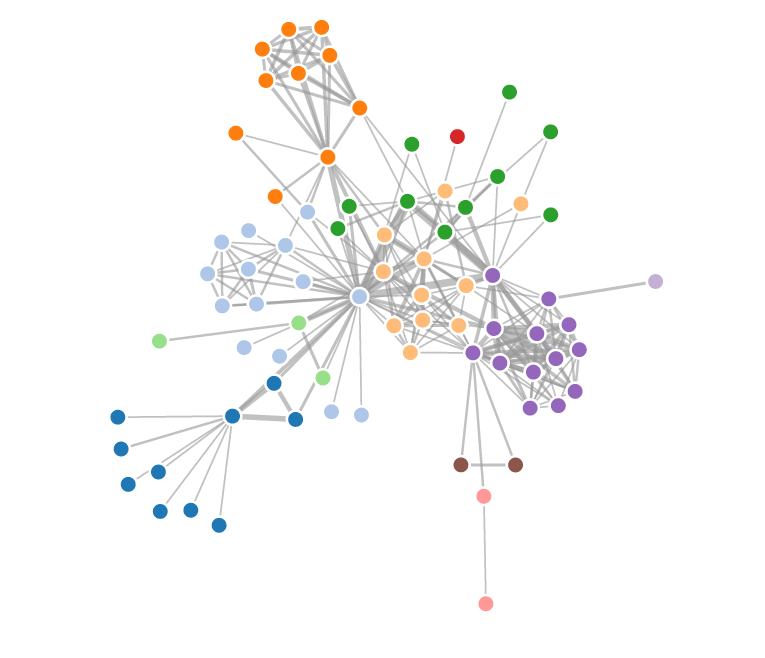
\includegraphics[width=\textwidth*4/5]{implementation/forceDirected.png}
		\caption{Force directed graph of web resources with their hyperlinks}
		\label{fig:forceDirected}
	\end{figure}
	\paragraph{}
	Many other visualisations can be created with this bidirectional mapping between visualisation elements and data elements and as we can see, the framework allows us to exploit very different dimensions of the same dataset in many completely different ways. This will help the users to find the correct information, or answer questions about the general structure of the metadata.
	
	\section{Interaction} \label{sec:Interaction}
	\paragraph{}
	Now that we know how to save and retrieve the data and visualise this data in many different ways, we need a way to allow the user to create the metadata and once the data is rendered the users need to be able to manipulate this data.
	\paragraph{}
	The users are able to create a selection on a web page using their cursor and save this selection as a \code{selector} to use as the source or destination of a hyperlink. To aid us with the management of user created selections we make use of \emph{Rangy}\footnote{\url{http://code.google.com/p/rangy/}}, a JavaScript library that supports many abstractions for creating, serialising and restoring user created selections.
	\paragraph{}
	First we want to allow the users to select a part of the web page which we can capture with the \code{getSelection} method \code{Rangy} provides us. The resulting object is an XPointer representation of the users' selection which we need to serialise to save it to the database. When we want to render the selection back on the web page again we need to de-serialise the saved selection and use the resulting selection object to add indicators on the web page on which we can apply CSS styles.\\
	\begin{lstlisting}[language=JavaScript]
		//saving
		var sel = rangy.getSelection();
		var serializedSel = rangy.serializeSelection(sel);

		//restoring
		var cssApplier = rangy.createCssClassApplier("Selection"});
		var sel = rangy.deserialiseSelection(serializedSel);
		cssAppier.applyToRange(sel);
	\end{lstlisting}
	\paragraph{}
	Now that we can save and serialise the users' selection we only need to allow the users to select a particular piece of text and choose whether the selected text is the source or destination of the hyperlink that is being created.

	\section{Concerns} \label{sec:Concerns}
		\paragraph{}
		In this section we will discuss the setbacks and issues we have encountered while developing the tool.
		\paragraph{Dynamic Content}
		More and more websites are becoming interactive where a single web page will generate different content based on some value in the users' cookies or some server-side parameters. If users create a selector on a resource which is defined by its URL this relation is saved in the database. When the users then visit the same web page the database will be queried for all relevant selectors and since we had saved one before we will find at least one. This selector is defined by the XPointer that is saved in the database but when the tool tries to render this XPointer on the generated content there is no guarantee that the XPointer is still valid. This problem is even more noticeable on so-called \dquote{Single Page Websites} where all the content is requested with AJAX(CITE) calls and is then dynamically loaded on the web page.
		\paragraph{Same Origin Policy}
		The Same Origin policy is an important security concept for a number of client side programming languages, most notably JavaScript. The policy states that only scripts originating from the same host as the web page itself, are allowed to be executed on that page. Being the same host is then defined in terms of the scheme, host name and port number of the web page. The issue with our tool is that our JavaScript will be requested from a different domain than the web pages. The tool request the content of a web page from its actual server to get the latest version of the content and with this content loaded in a frame we use our JavaScript to manipulate the DOM structure of the document. This will be blocked by the same origin policy which does not allow our scripts to run on the document structure of another web page.
		\paragraph{X-Frame-Options}
		The X-Frame-Option header that can be set by the server is a mechanism developed by Microsoft in January 2009. This header option is intended to protect users against click jacking attacks. Click jacking, or User Interface Redressing is a malicious technique of tricking a user to click on something different than what the user intended to click on. This is accomplished by loading the content of a legitimate website in a frame, and then rendering a transparent layer on top of the other web page. When the users try to click on the displayed web page they are actually clicking on the transparent layer, triggering unintentional behaviour. The main problem with this technique is that it is very hard to detect from the server's side. Imagine a malicious user sending a link to a video to someone else. But another valid page, for example a product page of Amazon is layered on top of the video. When the user then wants to click on the play button for the video, he is actually clicking on the buy button for Amazon. Since the user most likely has an authentication token stored in a cookie somewhere, the invisible layer is actually authenticated. There is no distinction between a legitimate click on the buy button, or a click jacking attack from the viewpoint of the Amazon server.
	\paragraph{}
	Because of this security issue Microsoft introduced the X-Frame-Option header. This option provides a partial server-side prevention mechanism against these attacks. If a server enables this header option the browser will detect this tag and notify the users that their page is loaded in a frame, prompting the user to open their website in a new window. As a result the website that is opened in the new website will always be directly served by the intended web page and the transparent layer will not be rendered on top of it any more. The X-Frame-Option header tag can have different values, such as DENY, SAMEORIGIN or ALLOW-FROM. These options will prevent the served page to be rendered in a frame entirely. Most big websites will enable this options when they do not want their website to be loaded in a frame. This poses a major problem for our tool since we are loading all the content of third party websites into a frame before running our JavaScript on the content. Large companies' websites like Google, Facebook, etc. will therefore just result in an empty frame the users request their pages.
	\section{Workarounds} \label{sub:Workarounds}
	\paragraph{}
	For some of the previously mentioned issues we can find solutions or temporary workarounds. In this section we elaborate on some of these solutions.
	\paragraph{Dynamic Content}
	To make the hyperlinks more robust the tool could save a hash of the document when the hyperlink is created. The next time the web page is loaded the tool could hash the web page again and check whether the saved hash and the generated one match. When the hashes match the tool can be fairly sure that the rendered content is the same content as the author created the hyperlink on and by extension the intended context of the hyperlink will most likely not have changed. When the hashes do not match the tool could filter the hyperlink before it is rendered.
	\paragraph{}
	This technique will almost never give a false positive, so if a link is actually rendered the tool can almost always be sure that the hyperlink is correct. The problem is that the slightest change on the web page will cause all hyperlinks that were created on the web page to be invalid. Since many web pages add advertisement on the web page that changes every time the users visit the page, the tool will almost never render any hyperlinks at all. The problem is that the check is way to strict.
	\paragraph{}
	A similar approach is to not hash the entire page but create a hash of the structure of the web page, ignoring all content of the page. This will allow the page to change some small details such as advertisements or titles and so forth without breaking all existing hyperlink. The down side is of course that the content can change and change the context on which the hyperlink was created. False positives are a possibility in this scenario but the reduced strictness will be beneficial in practice.
	\paragraph{}
	Another approach is to only hash a part of the web page when we take the list of ancestors of the node on which the hyperlink was created and hash the structure of this list of elements, we can be quite certain that if the hash matches next time, we have a valid hyperlink on that page. To maintain at least some of the context, the tool could also hash the content of the node on which the hyperlink was created. This will ensure that the text will at least have stayed the same. It might be the case that the position of the text changed on the web page but the hyperlink could still be valid.
	\paragraph{X-Frame-Options}
	When users request a web page the tool now opens a frame and sets the location to the appropriate URL. The tool can also send an AJAX request to the intended server requesting the content of the specific page. When the tool receives the response it will create a \code{div} element in which the content of the response will be rendered. This way the server will not know the page is loaded in another page and even if the X-Frame option is set, the page will still be loaded. This will work very well when requesting the needed pages but the problem is the original links on the web page will point to the real web page, and clicking these links are not handled by our tool. So the browser will forward the users to the actual page, where they will not be able to take advantage of the functionality of our tool.
	\paragraph{}
	One possible solution to this new problem is scraping the requested content for hyperlinks and wrapping them with JavaScript \code{onClick} handlers. But this is not a waterproof technique either since many websites employ JavaScript of their own to simulate hyperlinks as well. These hidden links will not be captured and still direct the users away from the tool.
	\paragraph{}
	An additional problem is when the users load two separate websites in two \code{div} elements. When the tool loads the websites in frames they are sandboxed which means that their CSS and JavaScript rules will not conflict with each other. When we request the data ourselves and render it in a \code{div} we need to manually sandbox the retrieved result. This is of course possible but it is quite complicated to do this correctly.
	\paragraph{}
		Because we needed to be able to test our application, we needed some short term workarounds. Most modern browsers can be customized rather easily to disable some of the security options. Since we know that disabling the Same Origin Policy feature will not harm us when we are working with our tool we can temporarily turn this feature of when testing our tool. In a real environment this is of course not a very good idea, and the policy was introduced with good reasons, and it should not be disabled lightly, it is therefore only a short term workaround that allowed us to develop the tool.
	\paragraph{}
	In the long run, when the tool is converted from a stand alone tool to a plugin that manages the hyperlinks between web pages in a general all purpose browser, the browser can manage its own policy. If this general browser allows its' plugins to use JavaScript on content that is not from the same domain this issue is solved without the security risk. Since this general browser no yet exists this solution is currently not feasible.
